\chapter{Separar misturas}\label{ch:g3:separating-mixtures}

Depois de uma tempestade, as poças da rua ficam marrons: água da chuva
\omterm{def:g2:mixing-and-dissolving:mix}{misturada} com terra, areia e pedacinhos de folhas. Mesmo assim, a água
que sai da torneira da cozinha é límpida, e ela também já foi chuva,
antes de correr para um rio. Como deixar a água barrenta limpa de novo?
O que foi \omterm{def:g2:mixing-and-dissolving:mix}{misturado} pode ser separado. Este capítulo mostra como, um
método de cada vez.

\begin{recall}
\omterm{def:g2:mixing-and-dissolving:mix}{Misturar} é juntar coisas diferentes. Um sólido como o açúcar ou o sal \omterm{def:g2:mixing-and-dissolving:dissolve}{se
dissolve} na água: ele some da vista, e o líquido límpido é uma solução.
Um sólido dissolvido continua lá: quando a água seca, o sólido fica para
trás. A areia e a terra não se dissolvem
(\cref{ch:g2:mixing-and-dissolving}).
\end{recall}

\section{Separar com a mão e peneirar}

Quando os pedaços de uma mistura são grandes o bastante para serem
vistos e pegos, o jeito mais simples de separá-los é com a mão: dá para
tirar as passas da granola uma por uma. Quando os pedaços são muitos,
uma peneira faz a separação por nós.

\begin{definition}[Peneiração]\label{def:g3:separating-mixtures:sieve}
A \emph{peneiração}\index{peneiracao@peneiração} é a separação dos pedaços de uma
mistura pelo tamanho, com uma peneira: uma tela ou uma placa cheia de
furos. Os pedaços pequenos passam pelos furos; os pedaços grandes ficam
na peneira.
\end{definition}

\begin{example}[Cascalho e areia]\label{ex:g3:separating-mixtures:gravel}
Um pedreiro sacode uma mistura de cascalho e areia em cima de uma
peneira. A areia fina passa e forma um monte embaixo; o cascalho fica na
tela.
\end{example}

\begin{omfigure}
\begin{tikzpicture}[font=\small]
  % the sieve: a mesh bowl
  \fill[pattern=crosshatch, pattern color=black!45] (-1.6,2.6) arc[start angle=180,
    end angle=360, x radius=1.6, y radius=0.7] -- cycle;
  \draw[black!70, line width=0.8pt] (-1.6,2.6) arc[start angle=180, end angle=360,
    x radius=1.6, y radius=0.7];
  \draw[black!70, line width=0.8pt] (-1.75,2.6) -- (1.75,2.6);
  \draw[black!70, line width=1.4pt] (1.75,2.6) -- (3.0,2.85);
  % gravel kept in the sieve
  \foreach \x/\y/\r in {-0.9/2.25/0.17,-0.45/2.12/0.2,0.05/2.08/0.18,0.5/2.13/0.21,
                        0.95/2.28/0.16,-0.2/2.42/0.15,0.3/2.43/0.17}
    \fill[black!45, draw=black!65] (\x,\y) circle (\r);
  % sand falling
  \foreach \x/\y in {-0.4/1.6,0.1/1.4,0.4/1.7,-0.15/1.15,0.25/1.0,-0.5/0.95,0.0/0.75}
    \fill[orange!60!brown] (\x,\y) circle (0.05);
  % the heap of sand in a bowl
  \fill[orange!45!brown!70] (-1.0,0.12) .. controls (-0.5,0.55) and (0.5,0.55)
    .. (1.0,0.12) -- cycle;
  \draw[black!70, line width=0.8pt] (-1.5,0.5) .. controls (-1.3,0) and (1.3,0)
    .. (1.5,0.5);
  \node[anchor=west] at (2.0,2.2) {o cascalho fica na peneira};
  \node[anchor=west] at (2.0,1.25) {a areia passa pelos furos};
  \node[anchor=west] at (2.0,0.3) {um monte de areia};
\end{tikzpicture}

{\small \omterm{def:g3:separating-mixtures:sieve}{Peneiração} de uma mistura de cascalho e areia: os pedaços são
separados pelo tamanho.}
\end{omfigure}

\begin{omfigure}
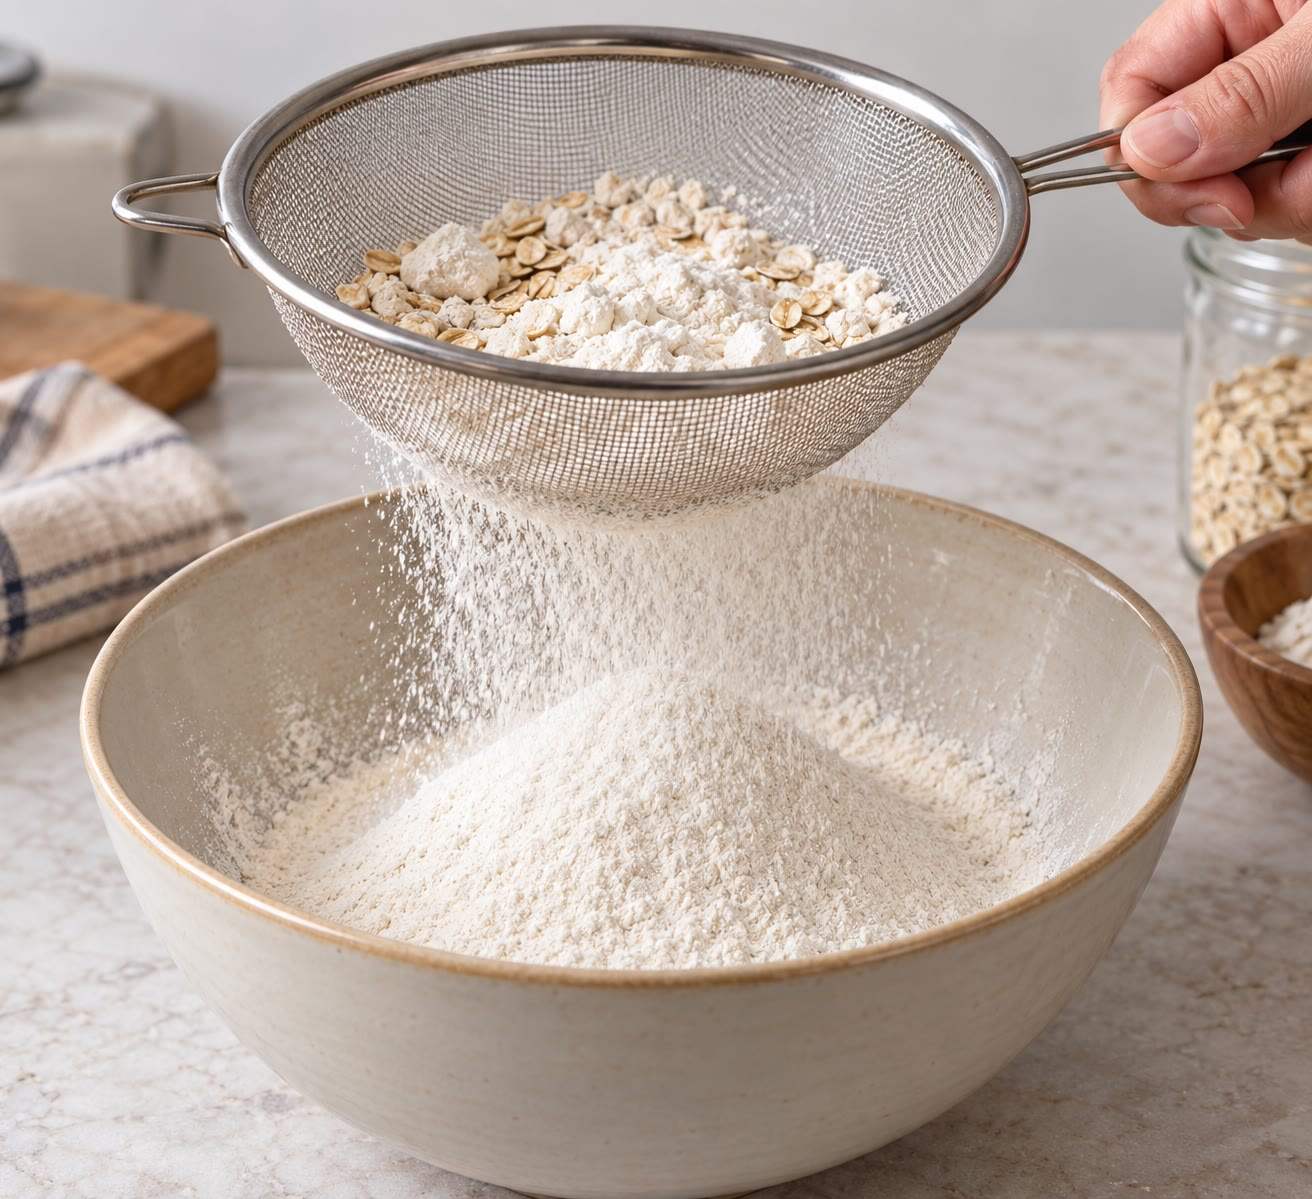
\includegraphics[width=0.55\linewidth]{images/book1/ai/g3-kitchen-sieve.jpg}

{\small Uma peneira de cozinha: a farinha fina passa, os grumos ficam
para trás.}
\end{omfigure}

\section{Deixar depositar e decantar}

\begin{definition}[Sedimentação e decantação]\label{def:g3:separating-mixtures:decant}
Uma mistura de água com um sólido que não \omterm{def:g2:mixing-and-dissolving:dissolve}{se dissolve} pode ser deixada
em repouso: o sólido desce devagar até o fundo. Isso se chama
\emph{sedimentação}\index{sedimentacao@sedimentação}. Depois que o sólido se
depositou, a água límpida de cima pode ser despejada com cuidado em
outro recipiente, deixando o sólido para trás: isso é a
\emph{decantação}\index{decantacao@decantação}.
\end{definition}

\begin{omfigure}
\begin{tikzpicture}[font=\small]
  % 1: stirred, cloudy
  \pic at (0,0) {beaker={0.7}{brown!28}};
  \foreach \x/\y in {-0.5/0.3,-0.2/0.6,0.3/0.4,0.5/0.9,-0.4/1.0,0.1/1.2,0.4/0.15,
                     -0.1/0.25,0.2/0.8,-0.55/0.7}
    \fill[brown!60] (\x,\y) circle (0.03);
  \node[anchor=north, align=center] at (0,-0.15) {mexida:\\ turva};
  \draw[->, thick, omProp] (1.1,1.0) -- (2.4,1.0);
  % 2: settled
  \pic at (3.5,0) {beaker={0.7}{omWater!80}};
  \fill[brown!60] (2.7,0) rectangle (4.3,0.25);
  \draw[omGlass, line width=0.7pt] (2.7,0.25) -- (2.7,0) -- (4.3,0) -- (4.3,0.25);
  \node[anchor=north, align=center] at (3.5,-0.15) {em repouso:\\ a terra se depositou};
  \draw[->, thick, omProp] (4.6,1.0) -- (5.9,1.0);
  % 3: decanted
  \pic at (7.0,0) {beaker={0.1}{omWater!80}};
  \fill[brown!60] (6.2,0) rectangle (7.8,0.25);
  \draw[omGlass, line width=0.7pt] (6.2,0.25) -- (6.2,0) -- (7.8,0) -- (7.8,0.25);
  \pic at (9.2,0) {beaker={0.58}{omWater!80}};
  \node[anchor=north, align=center] at (8.1,-0.15) {despejada: água límpida\\ à direita, a terra fica};
\end{tikzpicture}

{\small \omterm{def:g3:separating-mixtures:decant}{Sedimentação} e depois \omterm{def:g3:separating-mixtures:decant}{decantação} de uma mistura de terra e água.}
\end{omfigure}

\begin{remark}[A sedimentação leva tempo]\label{rem:g3:separating-mixtures:time}
Os grãos grandes e pesados se depositam em poucos minutos; uma argila
bem fina pode levar um dia ou mais, e enquanto isso a água continua um
pouco turva. A \omterm{def:g3:separating-mixtures:decant}{decantação} nunca tira todos os grãos: um pouco da
turvação vai embora junto com a água.
\end{remark}

\section{Filtrar}

\begin{definition}[Filtração e filtrado]\label{def:g3:separating-mixtures:filter}
A \emph{filtração}\index{filtracao@filtração} consiste em despejar uma mistura
através de um filtro: uma folha de papel, um pano ou uma camada de areia
com furos pequenos demais para deixar passar os pedaços sólidos. O
sólido fica no filtro; o líquido límpido que passa se chama
\emph{filtrado}\index{filtrado}.
\end{definition}

\begin{omfigure}
\begin{tikzpicture}[font=\small, scale=1.4]
  \pic[transform shape] at (0,0) {beaker={0.35}{omWater!80}};
  \pic[transform shape] at (0,1.4) {funnel={brown!55}};
  % muddy water waiting in the paper cone, above the soil
  \fill[brown!25] (-0.411,2.45) -- (0.411,2.45) -- (0.722,2.8) -- (-0.722,2.8) -- cycle;
  % drops of filtrate
  \foreach \y in {1.15,0.95} \fill[omDef!50] (0,\y) circle (0.04);
  \draw[<-, omProp, thick] (0.75,2.6) -- (2.0,2.9) node[right, text=black]
    {papel de filtro num funil};
  \draw[<-, omProp, thick] (0.25,2.15) -- (2.0,2.2) node[right, text=black]
    {a terra fica no papel};
  \draw[<-, omProp, thick] (0.85,0.4) -- (2.0,0.6) node[right, text=black]
    {o filtrado: água límpida};
\end{tikzpicture}

{\small \omterm{def:g3:separating-mixtures:filter}{Filtração} de água barrenta num filtro de papel.}
\end{omfigure}

\begin{inthelab}[Filtrar água barrenta]
O professor dobra uma folha redonda de papel de filtro em forma de cone
e a coloca num funil de vidro, em cima de um béquer. A água barrenta é
despejada no cone aos poucos, nunca acima da borda do papel. Uma água
límpida pinga no béquer; a terra forma uma camada marrom no papel. Se o
\omterm{def:g3:separating-mixtures:filter}{filtrado} sai turvo, é porque o papel rasgou ou a água passou por cima
da borda.
\end{inthelab}

\begin{proposition}[Um filtro não segura o que está dissolvido]\label{prop:g3:separating-mixtures:dissolved}
Um filtro segura os pedaços sólidos que não estão dissolvidos. Ele não
segura o que está dissolvido: a água salgada despejada num filtro sai
tão salgada quanto entrou, e o chá adoçado, tão doce quanto antes.
\end{proposition}

\begin{omfigure}
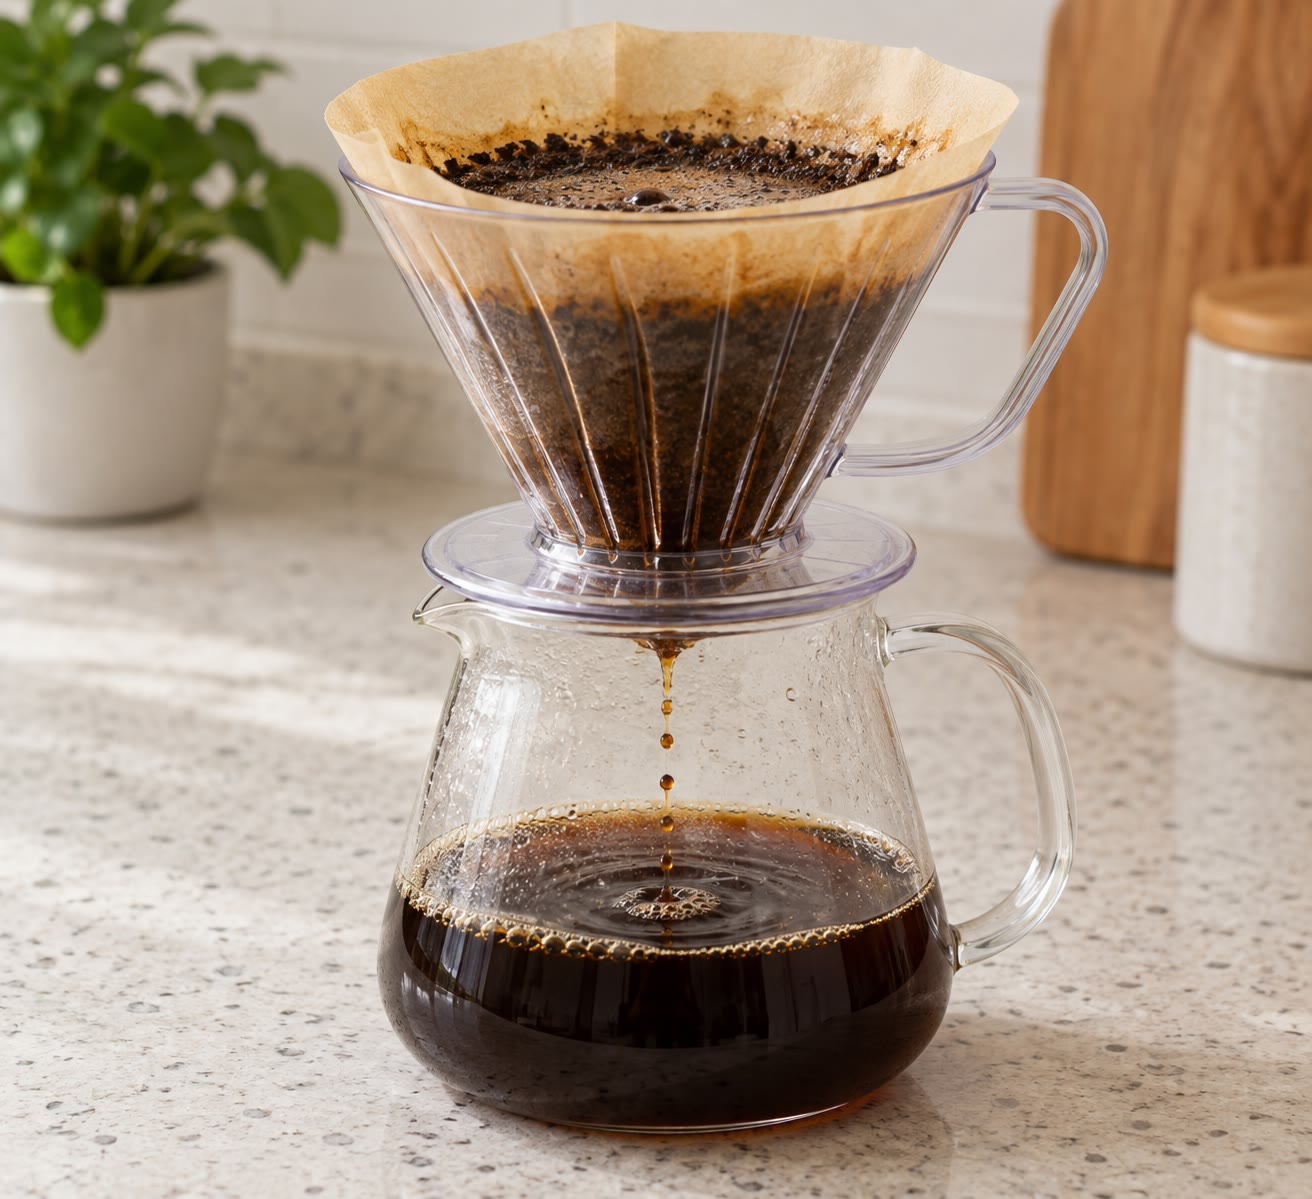
\includegraphics[width=0.5\linewidth]{images/book1/ai/g3-coffee-filter.jpg}

{\small Passar café é filtrar: o pó fica no papel, o café é o \omterm{def:g3:separating-mixtures:filter}{filtrado}.}
\end{omfigure}

\section{Fazer a água evaporar}

\begin{definition}[Evaporação]\label{def:g3:separating-mixtures:evaporate}
Para recuperar um sólido dissolvido na água, deixamos a água secar, no
sol ou num aquecimento suave: isso é a
\emph{evaporação}\index{evaporacao@evaporação}. A água vai para o ar; o sólido fica
no recipiente.
\end{definition}

\begin{example}[Sal a partir de água salgada]\label{ex:g3:separating-mixtures:salt}
Um pouco de água salgada é despejado num pratinho raso, deixado no
parapeito de uma janela ensolarada. Dias depois não sobra água nenhuma,
só uma crosta branca de sal: o sal que estava dissolvido.
\end{example}

\begin{omfigure}
\begin{tikzpicture}[font=\small, scale=1.4]
  \pic[transform shape] at (0,0) {hotplate};
  \pic[transform shape] at (0,0) {evapdish={omWater!80}};
  \node[anchor=north, align=center] at (0,-0.6) {água salgada,\\ aquecida devagar};
  \draw[->, thick, omProp] (1.5,0.3) -- (3.0,0.3) node[midway, above, text=black]
    {depois};
  \pic[transform shape] at (4.5,0) {hotplate};
  \pic[transform shape] at (4.5,0) {evapdish={white!85!black}};
  \foreach \x in {-0.45,-0.25,-0.05,0.15,0.35}
    \fill[white, draw=black!45, line width=0.2pt] (4.5+\x,0.12) rectangle ++(0.09,0.06);
  \node[anchor=north, align=center] at (4.5,-0.6) {sem água:\\ cristais de sal};
  \foreach \x in {-0.3,0,0.3} \draw[->, black!45, decorate,
    decoration={snake, amplitude=0.6pt, segment length=4pt}] (\x,0.7) -- (\x,1.4);
  \node[anchor=south] at (0,1.4) {a água vai para o ar};
\end{tikzpicture}

{\small A \omterm{def:g3:separating-mixtures:evaporate}{evaporação}, no laboratório: o professor aquece o recipiente
devagar numa placa de aquecimento. O sal fica no recipiente.}
\end{omfigure}

\section{Que método para que mistura?}

\begin{method}[Escolher uma separação]\label{met:g3:separating-mixtures:choose}
Para separar uma mistura, pergunte:
\begin{enumerate}
  \item Os pedaços são grandes e de tamanhos diferentes? Separe com a
        mão, ou peneire.
  \item Há um sólido que não \omterm{def:g2:mixing-and-dissolving:dissolve}{se dissolve}, dentro de um líquido? Deixe-o
        depositar e decante, ou filtre para ter uma água mais límpida.
  \item Há um sólido dissolvido no líquido? Faça o líquido evaporar: o
        sólido fica.
\end{enumerate}
Muitas vezes são necessárias várias etapas, uma depois da outra.
\end{method}

\begin{example}[Areia, sal e água]\label{ex:g3:separating-mixtures:three}
Um pote tem água com areia e sal. O sal se dissolveu; a areia, não.
\begin{enumerate}
  \item Filtre: a areia fica no papel.
  \item O \omterm{def:g3:separating-mixtures:filter}{filtrado} é límpido, mas é água salgada. Faça-o evaporar: o sal
        fica no recipiente.
\end{enumerate}
Dois métodos, um depois do outro, devolvem a areia e o sal.
\end{example}

\begin{example}[Água limpa a partir de um rio]\label{ex:g3:separating-mixtures:plant}
Uma estação de tratamento de água deixa a água do rio boa para beber em
várias etapas:
\begin{enumerate}
  \item a água do rio passa por grades, grandes telas que seguram
        galhos, folhas e plásticos: uma espécie de \omterm{def:g3:separating-mixtures:sieve}{peneiração};
  \item ela descansa em tanques grandes, onde a lama se deposita no
        fundo;
  \item ela é filtrada por camadas grossas de areia que seguram os grãos
        mais finos;
  \item é acrescentada uma quantidade bem pequena de um produto que mata
        os micróbios, para que a água continue segura nos canos.
\end{enumerate}
\end{example}

\begin{omfigure}
\begin{tikzpicture}[font=\small, node distance=0.45cm,
    box/.style={draw=omDef, fill=omDef!6, rounded corners=2pt, align=center,
      minimum height=1.15cm, text width=2.0cm}]
  \node[box] (r) {água\\ do rio};
  \node[box, right=of r] (s) {grades\\ (peneiração)};
  \node[box, right=of s] (t) {tanques de\\ sedimentação};
  \node[box, right=of t] (f) {filtros\\ de areia};
  \node[box, right=of f] (g) {micróbios\\ eliminados};
  \foreach \a/\b in {r/s,s/t,t/f,f/g} \draw[->, thick, omProp] (\a) -- (\b);
  \node[below=0.15cm of s, font=\footnotesize, align=center] {galhos,\\ plástico};
  \node[below=0.15cm of t, font=\footnotesize, align=center] {lama};
  \node[below=0.15cm of f, font=\footnotesize, align=center] {grãos finos};
  \draw[->, thick, omProp] (g.south) -- ++(0,-0.8) node[below] {para as torneiras};
\end{tikzpicture}

{\small As etapas de uma estação de tratamento de água. Embaixo de cada
etapa: o que ela retira.}
\end{omfigure}

\begin{omfigure}
\begin{minipage}[t]{0.48\linewidth}\centering
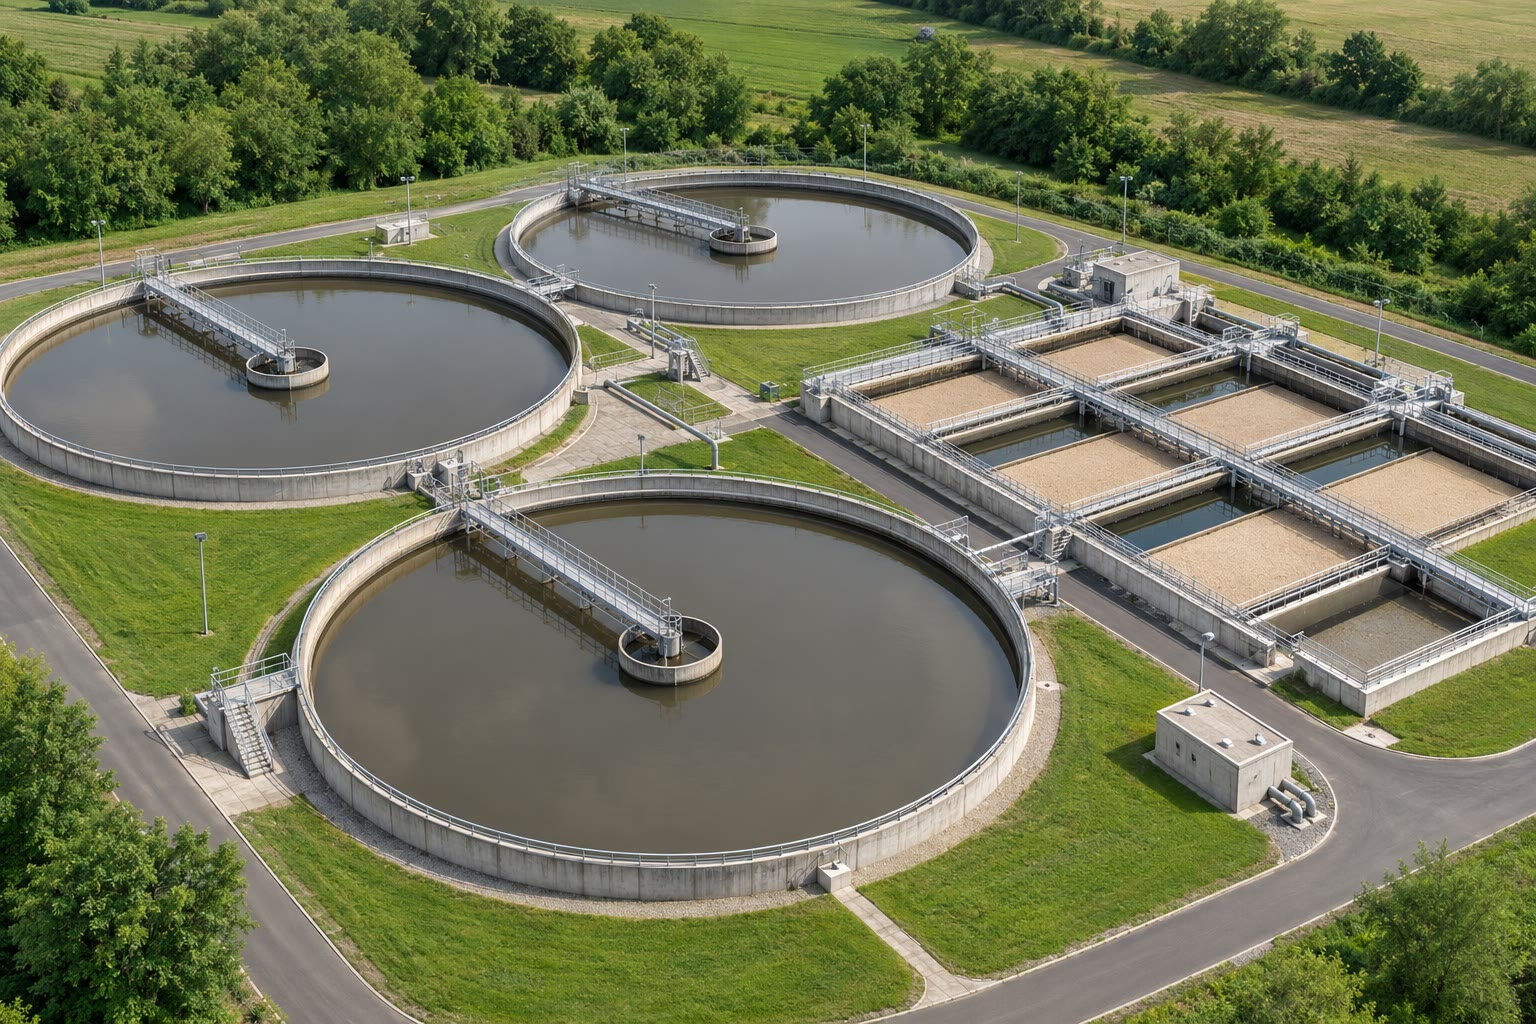
\includegraphics[width=\linewidth,height=4.6cm,keepaspectratio]{images/book1/ai/g3-settling-tanks.jpg}

{\small Tanques de \omterm{def:g3:separating-mixtures:decant}{sedimentação} de uma estação de tratamento de água.}
\end{minipage}\hfill
\begin{minipage}[t]{0.48\linewidth}\centering
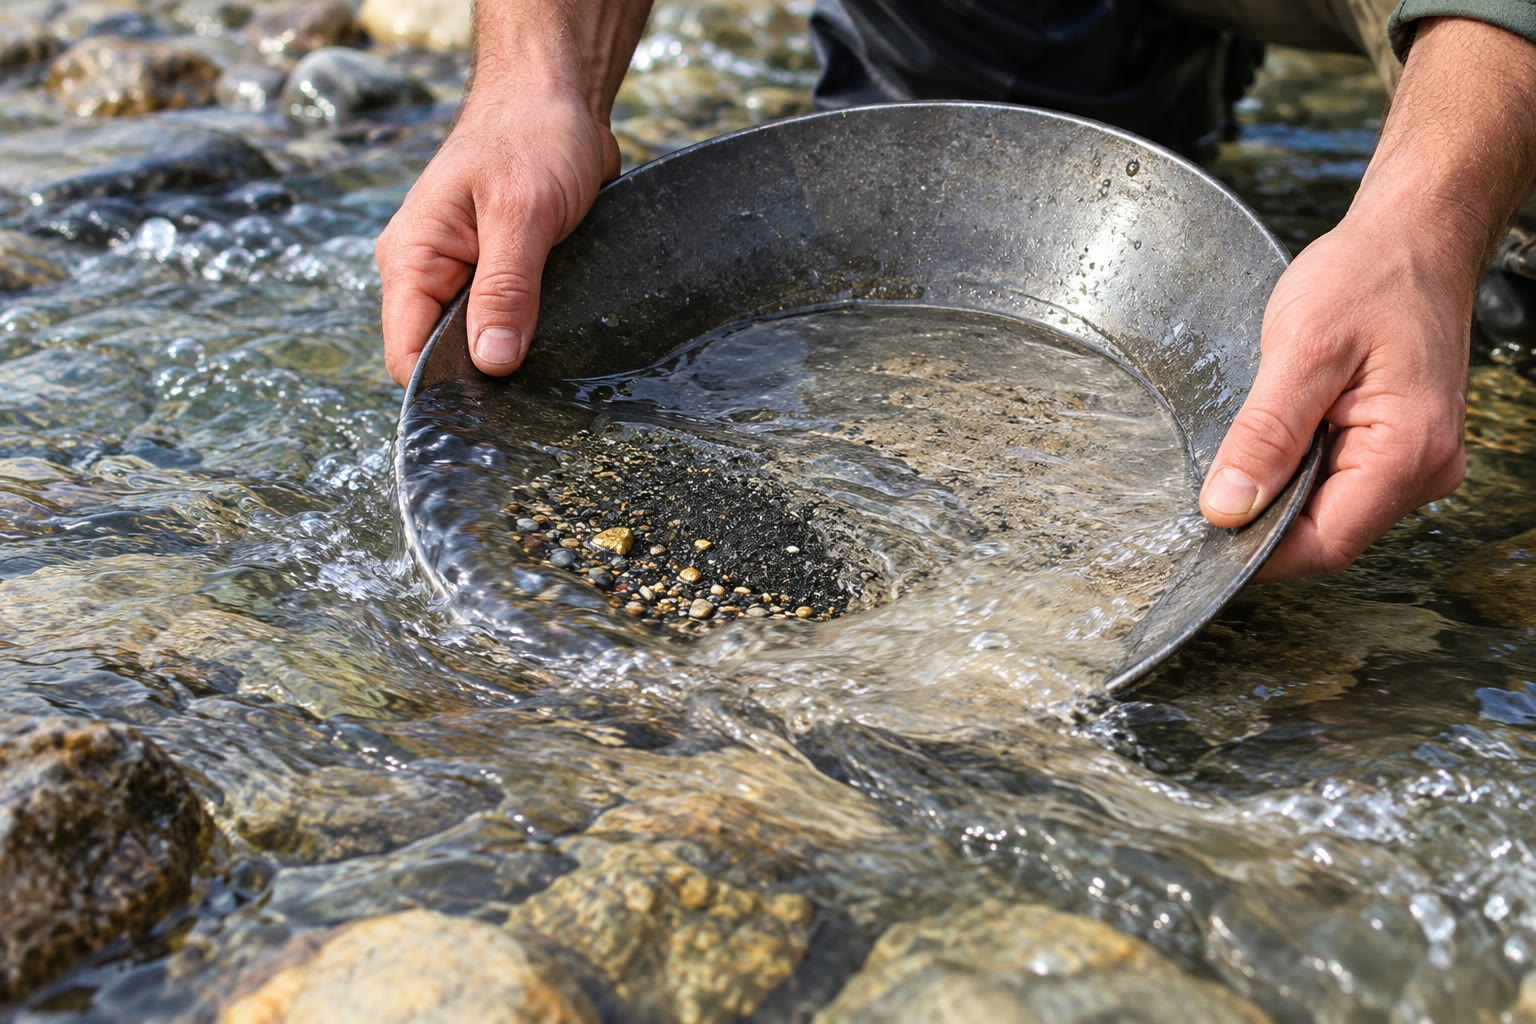
\includegraphics[width=\linewidth,height=4.6cm,keepaspectratio]{images/book1/ai/g3-gold-panning.jpg}

{\small Garimpo de ouro na bateia: a água do rio leva embora a areia
leve; os grãos pesados ficam na bateia.}
\end{minipage}
\end{omfigure}

\begin{remark}[Límpido nem sempre quer dizer limpo]\label{rem:g3:separating-mixtures:clean}
Uma água filtrada pode parecer perfeitamente límpida e ainda conter
substâncias dissolvidas, e micróbios pequenos demais para serem vistos.
É por isso que ninguém bebe a água de uma poça ou de um riacho, mesmo
depois de filtrá-la.
\end{remark}

\section{Exercícios}

\begin{exercise}[$\star$]\label{exo:g3:separating-mixtures:1}
Que método você usaria para separar ervilhas de grãos de arroz?
\end{exercise}

\begin{exercise}[$\star$]\label{exo:g3:separating-mixtures:2}
Um copo de água barrenta fica uma hora em cima de uma mesa. O que
acontece com a terra? Como isso se chama?
\end{exercise}

\begin{exercise}[$\star$]\label{exo:g3:separating-mixtures:3}
O que é um \omterm{def:g3:separating-mixtures:filter}{filtrado}? Diga qual é o \omterm{def:g3:separating-mixtures:filter}{filtrado} quando se passa um café.
\end{exercise}

\begin{exercise}[$\star$]\label{exo:g3:separating-mixtures:4}
Água salgada é despejada num papel de filtro. O \omterm{def:g3:separating-mixtures:filter}{filtrado} é salgado?
Explique.
\end{exercise}

\begin{exercise}[$\star$]\label{exo:g3:separating-mixtures:5}
Como recuperar o açúcar de um copo de água com açúcar?
\end{exercise}

\begin{exercise}[$\star$]\label{exo:g3:separating-mixtures:6}
Olhe a figura da peneira. Que pedaços ficam na peneira? Por que os
outros passam?
\end{exercise}

\begin{exercise}[$\star$]\label{exo:g3:separating-mixtures:7}
Ligue cada mistura a um método --- \omterm{def:g3:separating-mixtures:sieve}{peneiração}, \omterm{def:g3:separating-mixtures:filter}{filtração} ou \omterm{def:g3:separating-mixtures:evaporate}{evaporação}:
(a) areia e pedrinhas; (b) pó de giz na água; (c) sal na água.
\end{exercise}

\begin{exercise}[$\star$]\label{exo:g3:separating-mixtures:8}
Olhe a figura da estação de tratamento de água. Por quantas etapas a
água passa? Que etapa retira a lama?
\end{exercise}

\begin{exercise}[$\star$]\label{exo:g3:separating-mixtures:9}
Ponha estas etapas em ordem para recuperar a areia e o sal de um pote de
areia, sal e água: fazer o \omterm{def:g3:separating-mixtures:filter}{filtrado} evaporar; filtrar; recolher a areia
do papel.
\end{exercise}

\begin{exercise}[$\star\star$]\label{exo:g3:separating-mixtures:10}
Um filtro consegue deixar a água do mar boa para beber? Explique por
que não.
\end{exercise}

\begin{exercise}[$\star\star$]\label{exo:g3:separating-mixtures:11}
Folhas de chá ficaram num bule cheio de chá. Dê dois métodos, vistos
neste capítulo, que separam o chá das folhas.
\end{exercise}
